%!TEX root = Pflichtenheft.tex

\section{Produktübersicht}

% \begin{itemize}
% 	\item UML-Diagramme zu den Use-Cases hinzufügen
% \end{itemize}

% Repo erstellen und konfigurieren (Template, Rechnungsnummern, ...)
% Rechnung ausfüllen und erstellen (PDF, HTML, ...)
% Verwaltung der Rechnungen (offene Rechnungen, Statistiken, Analsye...)

% [Benutzer]-(Rechnung anlegen)
% [Benutzer]-(Rechnungsstatus ausgeben)
% [Benutzer]-(Rechnungsattribute bearbeiten)
% [Benutzer]-(Rechnung rendern)
% [Benutzer]-(Template konfigurieren)
% [Benutzer]-(Rechnungen durchsuchen)
% [Benutzer]-(Rechnung löschen)
% (Rechnung anlegen)<(Rechnungsattribute eingeben)
% (Rechnungsattribute bearbeiten)<(Rechnungsattribute eingeben)
% (Template konfigurieren)<(Platzhalter eintragen)
% http://yuml.me/5ed27f7e

\begin{center}
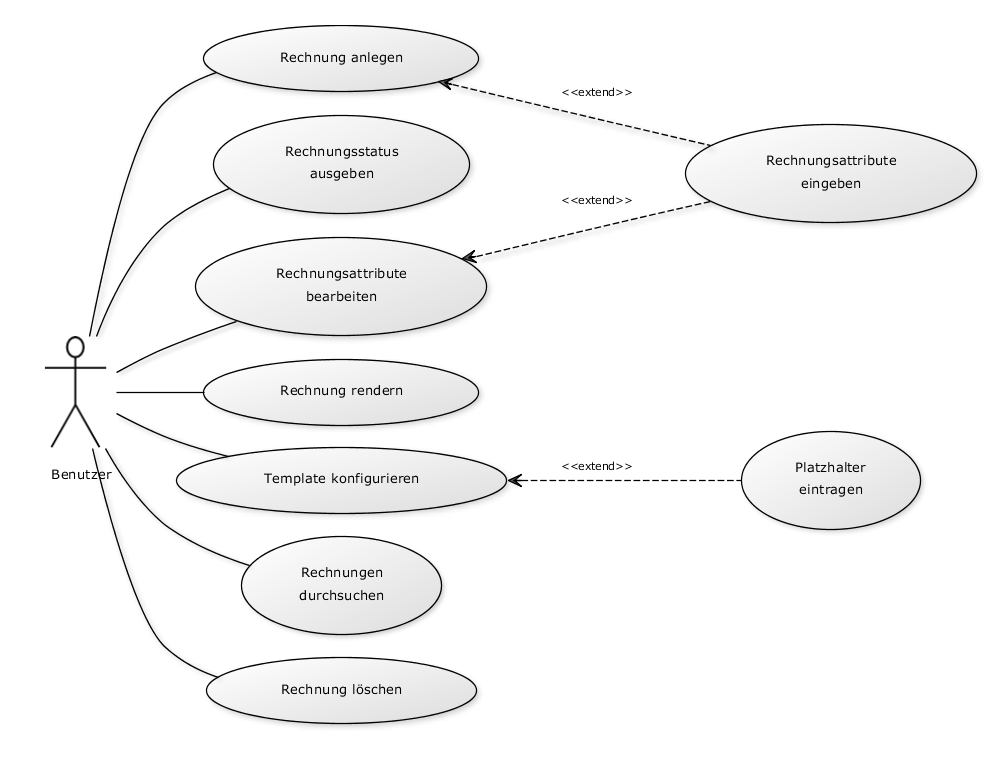
\includegraphics[width=0.8\textwidth]{03-Use-Case.png}
\end{center}